\documentclass[UTF8]{beamer}
\usepackage{graphicx, color}
\usepackage{algorithm2e}
\usepackage{zhspacing}
\usepackage{amsmath}

\usepackage{underscore}
\usetheme{JuanLesPins}
\usepackage{fontspec}
\setsansfont{Microsoft YaHei}

\usepackage{enumerate}

\AtBeginSection[]{
  \frame{
    \frametitle{Next}
    \tableofcontents[currentsection, subsectionstyle=show/shaded/hide]
  }
}

\AtBeginSubsection[]{
  \frame{
    \frametitle{Next}
    \tableofcontents[currentsubsection]
  }
}

\title{Python}

\author{Gang Chen\\ chengang@bgitechsolutions.com}

\logo{
\includegraphics[width=1.3cm]{bgi-logo.png}
\includegraphics[width=2.5cm]{cuhklogo.png}}
\date{\today}




\begin{document}

\begin{frame}
\titlepage
\end{frame}

\begin{frame}[t]\frametitle{Outline}
\tableofcontents[hideallsubsections]
\end{frame}

\section{Overview}

\begin{frame}
  \centerline{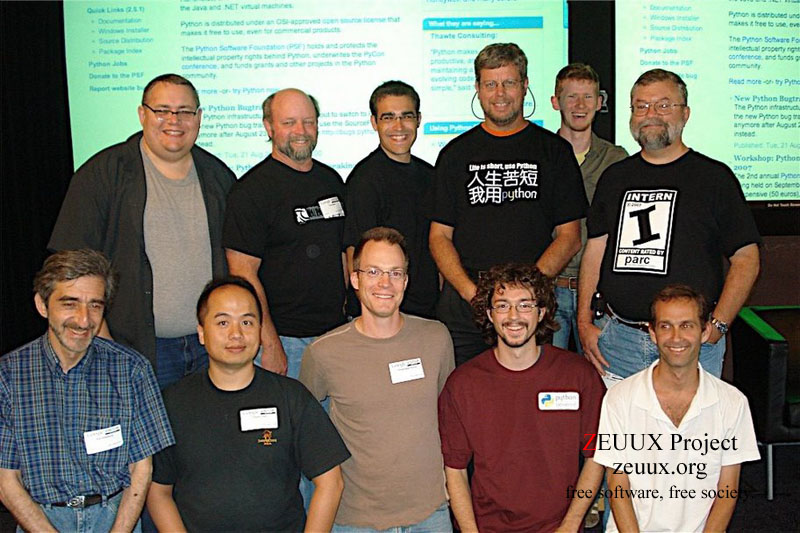
\includegraphics[height=\textheight]{guido.jpg}}
\end{frame}

\begin{frame}
  \centerline{\huge{Life is short}}
  \vspace{1cm}
  \centerline{\huge{You need Python!}}
  \vspace{1cm}
  \centerline{Bruce Eckel}
  \centerline{Author of \textit{Thinking in Java} and \textit{Thinking in C++}}
  \vspace{1.5cm}
  \centerline{\huge{人生苦短,我用Python}}
\end{frame}

\subsection{History}

\begin{frame}
  \frametitle{Brief History}
  \begin{itemize}
    \item December 1989, Guido wants a better ABC programming language
    \item October, 2000, Python 2.0 was released
    \item December, 2008, Python 3.0, a backwards-incompatible release, was
    released.
  \end{itemize}
\end{frame}

\begin{frame}
  \frametitle{Differences between Python 2 and 3}
  \begin{itemize}
    \item print is a function
    \item Views and iterators instead of lists
    \item 1/2 = 0.5; 1//2 = 0
    \item All text is unicode
    \item \ldots \ldots
  \end{itemize}
  Reference: https://docs.python.org/3/whatsnew/3.0.html
\end{frame}

\begin{frame}{Reference}
\begin{block}{Tutorials}
\begin{itemize}
  \item Google Python Class: https://developers.google.com/edu/python/?csw=1
  \item Official Documents: https://www.python.org/doc/
\end{itemize}
\end{block}

\begin{block}{Books}
  \begin{itemize}
    \item Lovely Python, 可爱的Python
    \item Think Python: How to think like a computer scientist\\
    http://www.greenteapress.com/thinkpython/thinkpython.html

  \end{itemize}
\end{block}
\end{frame}

\section{Quick Get Started}
\subsection{Download and Installation}
\begin{frame}
\begin{block}{Required Softwares}
  Required softwares will be listed on GitHub before the coming
  lecture.

  https://github.com/gangchen/CUHK-I2P
\end{block}
\end{frame}

\begin{frame}
  \frametitle{Interpreters}
  \begin{block}{Various Python Interpreters}
    \begin{itemize}
      \item CPython: Official interpreter
      \item JPython: for Java Virtual Machine
      \item Ironpython: for .Net platform
      \item PyPy: just-in-time compiler
      \item Python for S60: Nokia
    \end{itemize}
  \end{block}
\end{frame}

\subsection{Hello Python}
\begin{frame}[fragile]
  \begin{verbatim}
    #!/usr/bin/python

    print "Hello, Python!";
  \end{verbatim}
\end{frame}

\subsection{Python Shell}

\section{Syntax}

\section{iPython}


\end{document}
